\documentclass[12pt,titlepage]{article}
\usepackage[margin=1.25in]{geometry}
\usepackage{graphicx,amsmath,blindtext,enumitem,longtable,tabu,tabularx}

%% Variables definition
\newcommand{\vSubject}{Critical Thinking and Problem Solving}
\newcommand{\vSubtitle}{Advanced Problem Solving Skills}
\newcommand{\vName}{Dicha Zelianivan Arkana}
\newcommand{\vNIM}{2241720002}
\newcommand{\vClass}{1i}
\newcommand{\vDepartment}{Information Technology}
\newcommand{\vStudyProgram}{D4 Informatics Engineering}

%% [START] Tikz related stuff
\usepackage{tikz}
\usetikzlibrary{svg.path,calc,shapes.geometric,shapes.misc}
\tikzstyle{terminator} = [rectangle, draw, text centered, rounded corners = 1em, minimum height=2em]
\tikzstyle{preparation} = [chamfered rectangle, chamfered rectangle sep=0.75em, draw, text centered, minimum height = 2em]
\tikzstyle{process} = [rectangle, draw, text centered, minimum height=2em]
\tikzstyle{decision} = [diamond, aspect=2, draw, text centered, minimum height=2em]
\tikzstyle{data}=[trapezium, draw, text centered, trapezium left angle=60, trapezium right angle=120, minimum height=2em]
\tikzstyle{connector} = [line width=0.25mm,->]
%% [END] Tikz related stuff

%% [START] Fancy header related stuff
\usepackage{fancyhdr}
\pagestyle{fancy}
\setlength{\headheight}{15pt} % compensate fancyhdr style
\fancyhead{}
\fancyfoot{}
\fancyfoot[L]{\thepage}
\fancyfoot[R]{\textit{\vSubject - \vSubtitle}}
\renewcommand{\footrulewidth}{0.4pt}% default is 0pt, overline for footer
%% [END] Fancy header related stuff

%% [START] Custom tabular command related stuff
\usepackage{tabularx}
\newcommand{\details}[2]{
    #1 & #2  \\
}
%% [END] Custom tabular command related stuff

%% [START] Figure related stuff
\newcommand{\image}[3][1]{
    \begin{figure}[h]
        \centering
        \includegraphics[#1]{#2}
        \caption{#3}
        \label{#3}
    \end{figure}
}
%% [END] Figure related stuff

\begin{document}
\begin{titlepage}
    \centering
    \vfill
    {\bfseries\LARGE
        \vSubject\\
        \vskip0.25cm
        \vSubtitle
    }
    \vfill
    
\includegraphics[width=6cm]{images/polinema-logo.png}
    \vfill
    {
        \textbf{Name}\\
        \vName\\
        \vskip0.5cm
        \textbf{NIM}\\
        \vNIM\\
        \vskip0.5cm
        \textbf{Class}\\
        \vClass\\
        \vskip0.5cm
        \textbf{Department}\\
        \vDepartment\\
        \vskip0.5cm
        \textbf{Study Program}\\
        \vStudyProgram
    }
\end{titlepage}

\section*{Assignment A}
\begin{itemize}
    \item Perfect Pots is a company that manufactures ornamental plant pots. The company's expenses (rent, insurance, etc.) are \$15,000 per year.
    \item They employ four administrative staff (manager, accountant, sales director and secretary) with a total income of \$85,000 per year.
    \item The pots for sale are made by a number of skilled workers; each of which can make up to 5000 pots in a year and generate an income of up to \$20,000 per year.
    \item Materials, labor, and other capital are worth \$1000 per 10,000 pots
    \item {
        What is the profit variance of the company when viewed based on the number of pots made and sold based on the selling price of the pot 
        (assuming the company only makes pots for customers who order only)?

        First, we want to extract the data to make it easier to calculate.

        \begin{align*}
            Expenses &= \$15,000/year\\
            Fee &= \$85,0000/year\\
            Pot~sold &= 5000/year\\
            Income &= \leq\$20,000/year\\
            Materials,~labor,~other~capital &= \$1000~per~10,000~pots
        \end{align*}

        From the data above, we can say that each year, the company has an expense of \$100,000 (expenses + fee). Each pot, has 
        a production cost of \$0.1 because each year they sold \$5000 pots and the total cost for \$10,000 pots is \$1000. 
        So, 5000 pots will take $\frac{\$1000}{2}=\$500$ to produce and each pot will take $\frac{\$500}{5000}=\$0.1$ to produce.
        
        The company need to make at least \$100,000 each year to cover their total expense (rent, insurances, and staff salary).
        Which means, each pot need to have at least \$20 profit because each year there are 5000 pots sold which makes it $5000\times\$20=\$100,000$.

        To be in profit, they need to sell each pot ranging from \$20.1 to \$24.1. The \$0.1 is added because each pot has a production cost of \$0.1
        and its profit need to be at least \$20 to \$24 to reach \$0 to \$20,000 net profit.
    }
    \pagebreak
    \item {
        The graph in the right (Figure \ref{charitable_graph}) shows the types of charitable foundations in the UK that accept donations from the public.
        The total donations made by the community as a whole are estimated at \pounds11 billion Euros.

        \begin{figure}[h]
            \centering
            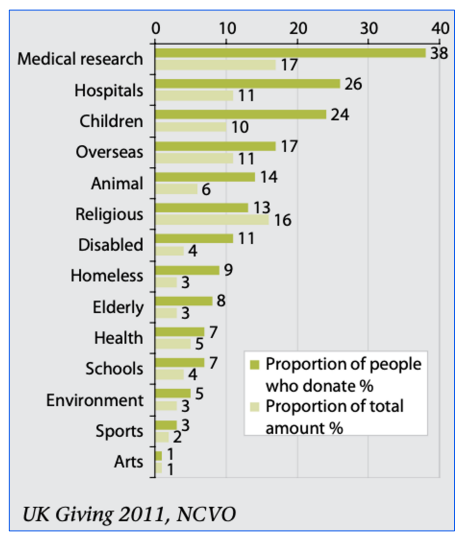
\includegraphics[width=7.5cm]{images/graph_1.png}
            \caption{Types of charitable foundation}
            \label{charitable_graph}
        \end{figure}
    }
    \item {
        While the types of donation sources for "medical charities" are shown in the pie chart below (Figure \ref{donation_graph}):

        \begin{figure}[h]
            \centering
            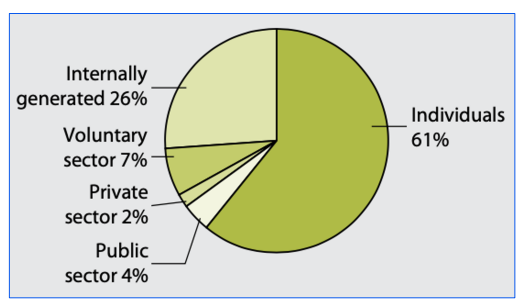
\includegraphics[width=8cm]{images/graph_2.png}
            \caption{Types of donation sources}
            \label{donation_graph}
        \end{figure}
    }
    \pagebreak
    \item {
        Answer the questions on the next slide and provide a brief explanation for each of your answers:

        \begin{enumerate}[label=\Alph*.]
            \item {
                Which types of charitable foundations do individual donors make the largest average contribution?

                We can see from the cart above the only organisation that has a proportion of total amount that exceeds the proportion of people donated is the Religious organisations, thus making it the answer.
            }
            \item {
                Which types of charitable foundations do individual donors make the smallest average amount of donations?

                The organisation that has the smallest average amount of donation is the homeless organisation because it has a 3:1 ratio of the proportion of people who donate to the proportion of total amount.
            }
            \item {
                What is the estimated total income of medical research charitable foundations?

                We can calculate the individual donations as such:
                \begin{align*}
                    17\%\times\pounds11~billion=\pounds1.87~billion
                \end{align*}
                The invididual donations only made up 61\% of the total donation. To find the total donation, we can divide the amount by the percentage like so:
                \begin{align*}
                    \pounds\frac{1.8}{0.61}~billion = \pounds3.07~billion
                \end{align*}
            }
            \item {
                It has been reported elsewhere that 6\% of all charitable foundations receive 90\% of the total
                donations, but "medical research" which is the recipient of the largest benefit, receives 17\% of the
                donations. Explain about this.

                The numbers on the chart do not relate to the charities, they only relate to the proportions.
            }
        \end{enumerate}
    }
\end{itemize}

\end{document}

